\subsection{\textit{Blockchain-Technologie}}

\subsubsection{Definition}


\subsubsection{Arten von \textit{Blockchain}}


\paragraph{Permissioned vs. Permissionless}


\paragraph{Public vs. Consortium vs. Private}


\subsubsection{Technologischer Aufbau}


\paragraph{Peer-to-Peer Netzwerke}


\paragraph{Signierte Transaktionen durch Public-Key-Infrastruktur}


\paragraph{Kryptographisches Hashing}


\paragraph{Konsensusprotokolle}


\subparagraph{Proof-of-Work}
\begin{figure}[h!]
	\centering
	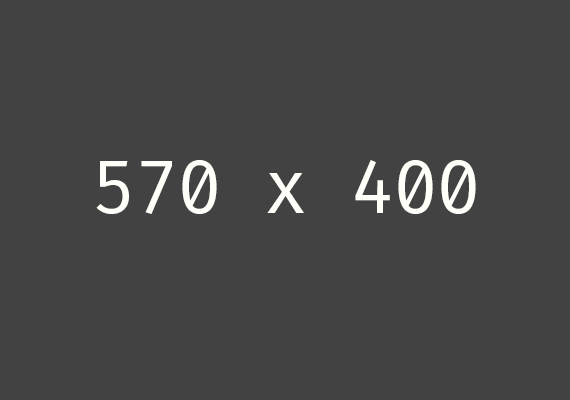
\includegraphics[width=1.0\linewidth]{pictures/placeholder_half_page}
	\caption[Placeholder Half Page]{Placeholder Half Page}
	\label{fig:placeholder_half_page}
\end{figure}

\subparagraph{Proof-of-Stake}
\begin{figure}[h!]
	\centering
	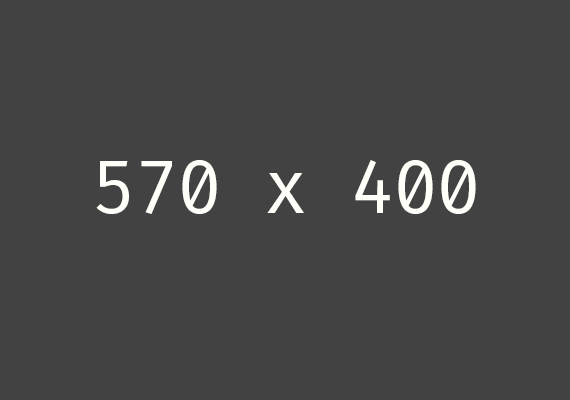
\includegraphics[width=1.0\linewidth]{pictures/placeholder_half_page}
	\caption[Placeholder Half Page]{Placeholder Half Page}
	\label{fig:placeholder_half_page}
\end{figure}

\subparagraph{Delegated Proof-of-Stake}
